\documentclass[11pt,a4paper]{article}
\usepackage[utf8]{inputenc}
\usepackage[T1]{fontenc}
\usepackage{lmodern}
\usepackage{hyperref}
\hypersetup{hidelinks}
\usepackage{graphicx}
\usepackage{listings}
\usepackage{xcolor}
\usepackage{booktabs}
\usepackage{amsmath}
\usepackage{geometry}
\usepackage{natbib}
\usepackage{fancyhdr}
\usepackage{float}
\usepackage{subcaption}
\usepackage{multirow}

\geometry{margin=1in}

\definecolor{codegreen}{rgb}{0,0.6,0}
\definecolor{codegray}{rgb}{0.5,0.5,0.5}
\definecolor{codepurple}{rgb}{0.58,0,0.82}
\definecolor{backcolour}{rgb}{0.95,0.95,0.92}

\lstdefinestyle{pythonstyle}{
    backgroundcolor=\color{backcolour},   
    commentstyle=\color{codegreen},
    keywordstyle=\color{magenta},
    numberstyle=\tiny\color{codegray},
    stringstyle=\color{codepurple},
    basicstyle=\ttfamily\footnotesize,
    breakatwhitespace=false,         
    breaklines=true,                 
    captionpos=b,                    
    keepspaces=true,                 
    numbers=left,                    
    numbersep=5pt,                  
    showspaces=false,                
    showstringspaces=false,
    showtabs=false,                  
    tabsize=2,
    language=Python
}

\lstset{style=pythonstyle}

\title{\textbf{AMBER: A Columnar Architecture for High-Performance Agent-Based Modeling in Python}}

\author{Anh-Duy Pham\\
\small University of Würzburg, Germany\\
\small \texttt{ORCID: 0000-0003-3832-9453}
}

\date{May 2026}

\begin{document}

\maketitle

\begin{abstract}
AMBER (Agent-based Modeling with Blazingly Efficient Records) is a Python framework for large-scale agent-based simulation. Unlike conventional Python ABM frameworks that store each agent as a Python object, AMBER centralises agent state in a columnar DataFrame backed by Polars and exposes it through a vectorised \emph{view API} (\texttt{agents.where(...)}, \texttt{agents.at[ids]}, \texttt{scatter\_add}) that lets domain scientists express population-wide updates in a handful of expressions. An explicit object-oriented escape hatch remains available for per-agent logic that does not vectorise. Benchmarked against six other frameworks (Mesa, AgentPy, SimPy, Melodie, Agents.jl, and AMBER's own OOP path) with output-invariant verification, AMBER is the fastest Python-hosted framework on every tested model, reaching speedups of up to 1118$\times$ over Mesa and beating the Julia-based Agents.jl on the largest SIR benchmark.
\end{abstract}

\vspace{1em}
\noindent\textbf{Keywords:} agent-based modelling; Python; columnar data; Polars; high-performance simulation; scientific software

\tableofcontents
\newpage

\section{(1) Overview}

\subsection{Introduction}

Agent-based modelling (ABM) studies complex adaptive systems by simulating autonomous agents whose local interactions generate emergent macro-level phenomena \citep{abar2017agent}. The methodology is central to computational epidemiology, ecology, economics, and social simulation, where it captures agent heterogeneity, spatial structure, and adaptive behaviour in ways that aggregate equation-based models cannot.

Python has become the dominant platform for ABM in the research community, primarily through the Mesa \citep{masad2015mesa} and AgentPy \citep{foramitti2021agentpy} frameworks. Their accessibility has enabled widespread adoption, but both---along with nearly every other Python-hosted ABM tool---share an architectural assumption that limits their scalability: each agent is a Python object, and each population-wide update is a Python-level \texttt{for} loop over those objects. For populations of thousands to tens of thousands of agents---scales typical in epidemiological and ecological modelling---the interpreter overhead of this pattern becomes the dominant cost, constraining parameter sweeps, Monte Carlo replicates, and model complexity.

AMBER (Agent-based Modeling with Blazingly Efficient Records) resolves this tension through two complementary architectural choices. First, agent state is centralised in a columnar DataFrame backed by Polars \citep{polars_zenodo}, a high-performance data processing library implemented in Rust. Second, a \emph{view API} (\texttt{model.agents.where(predicate)}, \texttt{model.agents.at[ids]}, \texttt{view.scatter\_add(**deltas)}) compiles user-facing update expressions down to a handful of Polars operations, giving domain scientists an intuitive idiom that nonetheless executes entirely in compiled code. A traditional object-oriented \texttt{Agent} class remains available as an escape hatch for per-agent logic that does not vectorise.

\subsection{Statement of Need}

Researchers who build large ABMs currently face a binary choice. They can stay in Python and accept the interpreter-overhead ceiling of Mesa or AgentPy, or they can migrate to a compiled language---Java (Repast \citep{north2013complex}, MASON \citep{luke2005mason}), Julia (Agents.jl \citep{datseris2024agents}), or GPU-accelerated C++ (FLAME GPU 2 \citep{richmond2023flame})---and pay the cost of learning a second language and maintaining a second toolchain. The first choice caps realistic population sizes; the second fragments a lab's codebase across languages and excludes collaborators without deep engineering expertise.

AMBER fills the gap by keeping the Python developer experience of Mesa and AgentPy while matching the performance of compiled alternatives for the workloads that most ABM researchers actually run. Users write Python; the framework executes Rust. Models already expressed in Mesa or AgentPy translate cleanly because AMBER preserves the \texttt{Model}/\texttt{Agent}/\texttt{AgentList} abstractions; the main change is that updates are expressed as views over the population rather than as loops over individual agents. Existing per-agent code continues to work through a buffered write path that is itself compiled into batched hash-join updates.

\subsection{Related Software}

\subsubsection{Python ABM Frameworks}

Mesa \citep{masad2015mesa} established the dominant Python ABM pattern: agents as Python class instances organised by a scheduler. It introduced widely-adopted idioms including datacollectors for state recording and modular space classes. Its design prioritises accessibility and flexibility, making it the default teaching and prototyping framework.

AgentPy \citep{foramitti2021agentpy} refines Mesa's approach with improved ergonomics, tighter Jupyter integration, and a built-in parameter-sweep \texttt{Experiment} API. Its \texttt{AgentList} exposes aggregate operations over collections, though the underlying storage is still object-per-agent.

Melodie \citep{yu2023melodie} separates models into agents, environment, scenario, and calibrator components, accelerating hot paths through Cython compilation. ABSESpy \citep{wang2024absspy} extends Mesa with domain-specific abstractions for social-ecological systems modelling. SimPy \citep{zinoviev2024discrete} is a discrete-event simulation library: not an ABM framework per se, but included here as a high-performance Python baseline since it is sometimes repurposed for agent simulation.

\subsubsection{Compiled-Language ABM Frameworks}

Repast \citep{north2013complex} and MASON \citep{luke2005mason} are mature Java-based platforms offering sophisticated scheduling, GIS integration, and checkpointing. Agents.jl \citep{datseris2024agents} leverages Julia's JIT compilation and multiple dispatch to combine scripted development with compiled execution; it is the direct non-Python performance baseline in our evaluation. FLAME GPU 2 \citep{richmond2023flame} maps agent operations onto CUDA kernels for GPU-accelerated simulation at massive scale but requires CUDA expertise and GPU-amenable model structure. NetLogo \citep{tisue2004netlogo} remains influential for its visual development environment and domain-specific language.

\subsubsection{Columnar Data Processing}

Columnar storage---organising data by columns rather than rows---has revolutionised analytical database systems and scientific data processing \citep{arrow2026}. Modern CPUs favour contiguous memory access, SIMD instructions process multiple values per cycle, and column operations parallelise naturally. Polars \citep{polars_zenodo}, built on Apache Arrow's columnar memory format and implemented in Rust, exposes these capabilities through a Python-accessible DataFrame API with multi-threaded execution. AMBER's contribution is applying these database-oriented techniques to the distinct access patterns of agent-based simulation and hiding them behind an ABM-native abstraction.

\section{(2) Implementation and Architecture}

This section describes AMBER's implementation, starting from the columnar backend, building up through the view API that users actually write, and closing with the complementary components (environments, experiments, optimisation).

\subsection{From Objects to Columns}

Conventional ABM frameworks represent each agent as a Python object on the heap, with attributes stored in the object's \texttt{\_\_dict\_\_} and the population held as a list or dictionary of such objects. Memory is scattered: adjacent list entries point to distant heap addresses, and reading a single attribute across $N$ agents performs $N$ independent pointer-chase-and-hash-lookup operations. A population-wide update such as incrementing every agent's wealth becomes $N$ bytecode-interpreted iterations, each paying Python's overhead for reference counting, type checking, and dictionary access. Profiling reveals that for simple attribute updates, interpreter overhead dominates the actual computation by more than two orders of magnitude.

AMBER replaces this with a single Polars DataFrame in which each agent attribute occupies a contiguous typed column, and agents are identified by a sequential integer id. A population-wide read traverses one cache-friendly array; a population-wide write lowers to one SIMD-vectorised Polars operation. The architectural difference is not merely a performance optimisation but a shift in what it means for agent state to exist: the DataFrame is the single source of truth, and Python-level \texttt{Agent} instances (when they exist at all) are views over rows rather than containers of state.

\subsubsection{Columnar State Management}

AMBER restructures state storage fundamentally. All agent state resides in a single \texttt{Population} object that wraps a Polars DataFrame where each attribute is a column. Column data is stored in contiguous typed arrays (for example, an Int64 array for integer attributes), with rows corresponding to agents identified by sequential integer IDs.

A population-wide update becomes a single vectorized operation expressed through AMBER's \emph{view API}:

\begin{lstlisting}[caption={Vectorized population-wide update via the view API}]
# Increment wealth for every agent in a single operation
self.agents.wealth += 10
\end{lstlisting}

This assignment invokes a single Python-to-Rust call. The left-hand side \texttt{self.agents.wealth} returns a Polars Series sourced from the population DataFrame; the arithmetic executes in compiled Rust, and the assignment lowers to one \texttt{df.with\_columns(...)} call that replaces the column in place. For subset updates, the same syntax extends naturally:

\begin{lstlisting}[caption={Subset-conditional update via a filtered view}]
# Only agents with positive wealth give away one unit
donors = self.agents.where(self.agents.wealth > 0)
donors.wealth -= 1
\end{lstlisting}

The \texttt{where} call returns a \texttt{FilteredAgentList} view keyed by the ids matching the predicate; the subsequent assignment applies the update to exactly those rows via a single hash-join against the population DataFrame. No Python-level loop is ever materialized.

For id-indexed updates where an agent may appear multiple times (for example, scattering resources from $k$ donors to $k$ randomly chosen recipients), AMBER provides a \texttt{scatter\_add} primitive:

\begin{lstlisting}[caption={Id-indexed accumulate with duplicate handling}]
# Each donor picks a random recipient; credits accumulate correctly
# when two donors happen to choose the same agent.
recipients = self.nprandom.choice(self.agents.ids.to_numpy(),
                                  size=len(donors))
self.agents.at[recipients].scatter_add(wealth=1)
\end{lstlisting}

\texttt{scatter\_add} uses a numpy \texttt{np.add.at} fast path with a cached id-to-row-position lookup, handling duplicate ids correctly (summing their contributions rather than overwriting) while still executing in a single pass over the affected rows.

\subsection{When the Columnar Approach Wins}

Let $T_{OOP} = N \cdot (c_{iter} + c_{dict} + c_{op})$ be the cost of a population-wide attribute update in an object-oriented framework, where $c_{iter}$ and $c_{dict}$ are Python iteration and dictionary-access overheads and $c_{op}$ is the actual operation cost. Let $T_{col} = c_{call} + (N/k) \cdot c_{op}$ be the same cost in a columnar framework, where $c_{call}$ is the fixed cost of invoking a vectorised operation and $k$ is the SIMD parallelism factor. The speedup is $S \approx k \cdot (c_{iter} + c_{dict}) / c_{op}$ for large $N$ with simple operations, predicting that the columnar approach provides its largest advantage on cheap operations applied to large populations. This prediction is confirmed empirically in Section~\ref{sec:evaluation}, where AMBER's advantage over Mesa ranges from 23$\times$ on random walk to 1118$\times$ on population-wide wealth transfer.

\subsubsection{Agent-Specific Operations}

Not all ABM operations benefit from columnar storage. Many SIR-style infection rules, Schelling-style satisfaction checks, and graph-traversal behaviors are naturally expressed as conditional logic over each agent's local neighborhood. AMBER preserves an explicit escape hatch for these cases via the traditional \texttt{Agent} class:

\begin{lstlisting}[caption={Per-agent logic using the OOP escape hatch}]
class InfectedAgent(am.Agent):
    def step(self):
        neighbors = self.get_neighbors(pl.col("status") == "S")
        if neighbors.height > 0 and self.model.random.random() < 0.1:
            # Per-agent record; buffered and flushed in one join.
            neighbors[0].record("status", "I")
\end{lstlisting}

Per-agent \texttt{record} and \texttt{update\_data} calls do not fall off the performance cliff: AMBER's \texttt{Model} class buffers them into a \texttt{\_pending\_writes} dictionary and flushes the entire step's worth of updates via a single \texttt{df.update(on='id')} hash join on the next read of \texttt{agents\_df}. This turns the classical object-oriented \texttt{for agent in model.agents: agent.step()} pattern into an O(1) DataFrame clones per step rather than O(N).

\subsection{The View API}

A naive columnar implementation would sacrifice the intuitive agent-oriented programming model. AMBER addresses this through a \emph{view API} that wraps the underlying Polars DataFrame in three view types, each honoring the same attribute protocol:

\begin{itemize}
\item \texttt{AgentList} --- the full-population view, reachable as \texttt{model.agents}.
\item \texttt{FilteredAgentList} --- a predicate-defined subset, returned by \texttt{agents.where(expr)} or \texttt{agents[boolean\_mask]}.
\item \texttt{ScatterAgentList} --- an id-indexed subset (where ids may repeat), returned by \texttt{agents.at[ids]}.
\end{itemize}

All three views share the same contract: a column attribute read returns a \texttt{pl.Series} sourced from \texttt{model.agents\_df}, and a column attribute assignment queues through the same batched flush path. The DataFrame is the single source of truth; there is no Python-attribute shadow copy, which eliminates an entire class of stale-read bugs common in object-per-agent frameworks.

Predicates accept either a boolean Polars Series or a raw Polars expression, so the full Polars expression language is available without forcing domain scientists to learn it. For example, \texttt{self.agents.wealth > 0} (a Series-returning comparison) and \texttt{pl.col("wealth") > 0} (an expression tree) are both valid arguments to \texttt{where}.

The \texttt{Model} class complements the view API with a columnar bulk-create helper, \texttt{add\_agents(n, **columns)}, which initializes $n$ agents in a single call accepting per-column scalar broadcasts, lists, numpy arrays, or Polars Series. This eliminates the \texttt{for i in range(n): self.add\_agent(AgentClass(i))} pattern that would otherwise dominate setup time for large populations.

The \texttt{Population} class remains accessible as the lower-level columnar foundation, exposing \texttt{batch\_update\_by\_ids}, \texttt{batch\_add\_agents}, and \texttt{batch\_update} with a selector expression. Framework extension authors and performance-sensitive users can drop down to this layer; the view API is built on top of it.

\subsection{State Evolution Semantics}

ABM requires mutable state evolution over simulation time. AMBER supports both synchronous and asynchronous update semantics.

In synchronous (simultaneous) updates, all agents act on a consistent state snapshot. This mode enables full vectorization, as entire columns can be transformed simultaneously based on current values without interference between agents.

In asynchronous (sequential) updates, agents observe effects of prior agents' actions within the same time step. This mode is necessary for some model semantics but limits vectorization, as each agent's computation may depend on modifications made by previously processed agents.

\subsection{Framework Components}

Beyond the core columnar architecture and view API, AMBER provides the infrastructure a full ABM workflow requires.

\textbf{Spatial environments.} Three environment classes share a unified interface. \texttt{GridEnvironment} implements discrete $n$-dimensional lattices with Moore or von Neumann neighbourhoods and optional torus wrapping; agent positions are stored as integer columns in the Population DataFrame, enabling vectorised neighbour queries. \texttt{SpaceEnvironment} provides continuous $n$-dimensional spaces with radius-based neighbour queries; for large populations it integrates with \texttt{SpatialIndex} (a \texttt{scipy.spatial.cKDTree} wrapper) for $O(\log N)$ lookups. \texttt{NetworkEnvironment} integrates NetworkX for graph-based connectivity and ships built-in generators for Erd\H{o}s-R\'{e}nyi, Watts-Strogatz, and Barab\'{a}si-Albert topologies.

\textbf{Experiment management.} The \texttt{Experiment} class defines parameter spaces using \texttt{Sample} for discrete values and \texttt{IntRange} for integer ranges, generates Cartesian products over all combinations, supports configurable replication counts, and aggregates results directly into columnar form for downstream analysis. \texttt{ParallelRunner} provides multiprocessing-based parallel execution for independent simulations with near-linear speedup across CPU cores.

\textbf{Optimisation and calibration.} AMBER ships a hierarchy of optimisation strategies: grid search for low-dimensional discrete spaces, random search for high-dimensional exploration, Gaussian-process-based Bayesian optimisation for sample-efficient calibration, and integration with Sequential Model-based Algorithm Configuration (SMAC) for multi-fidelity and multi-objective optimisation.

\section{(3) Empirical Evaluation}
\label{sec:evaluation}

We evaluate AMBER against six other agent-based modeling frameworks through systematic benchmarking with a dedicated correctness audit that verifies all framework implementations compute equivalent models before timing.

\subsection{Experimental Design}

\subsubsection{Frameworks Compared}

We compare seven framework implementations. \textbf{AMBER (vectorized)} uses the view API described in Section~3. \textbf{AMBER (loop)} uses AMBER's object-oriented escape hatch (\texttt{Agent.record()} / \texttt{update\_data()}) and provides an apples-to-apples baseline at the OOP abstraction level. \textbf{Mesa} \citep{masad2015mesa} and \textbf{AgentPy} \citep{foramitti2021agentpy} are the two mainstream Python ABM frameworks. \textbf{SimPy} \citep{zinoviev2024discrete} is included as a discrete-event alternative with a tight C-based event-loop core. \textbf{Melodie} \citep{yu2023melodie} represents Cython-accelerated Python ABM. \textbf{Agents.jl} \citep{datseris2024agents} provides a Julia JIT-compiled baseline outside the Python ecosystem.

\subsubsection{Benchmark Models}

We selected three models representing different computational patterns. The \textbf{Wealth Transfer} model has each agent with positive wealth transfer one unit to a randomly selected other agent at each step. This workload is dominated by attribute reads and writes and represents the simplest workload profile for vectorization.

The \textbf{SIR Epidemic} model places agents in continuous 2D space (100$\times$100) where they transition between Susceptible, Infected, and Recovered states based on contact with infected neighbors within a fixed radius (5 units), transmission probability 0.1, and recovery time 14 steps. Five agents begin in the Infected state. This workload involves all-pairs spatial distance computation (quadratic in population size) and state-transition logic.

The \textbf{Random Walk} model has agents move in continuous 2D space using independent uniformly sampled $x$ and $y$ displacements with boundary clamping. This tests position update kernels that are fully vectorizable.

\subsubsection{Correctness Verification}

Runtime numbers are meaningful only if every framework is computing the same thing. Before any timing runs, we execute each framework against a dedicated correctness script, \path{benchmarks/correctness_check.py}, that checks per-model output invariants:

\begin{itemize}
\item \textbf{Wealth transfer}: total wealth must equal $N \cdot w_{init}$ at any step (Boltzmann conservation).
\item \textbf{Random walk}: all agent coordinates must lie within the configured world bounds (boundary clamp integrity).
\item \textbf{SIR epidemic}: the cardinalities $|S| + |I| + |R|$ must equal $N$ at every step, and the initial infected count must match the configured \texttt{initial\_infected} parameter.
\end{itemize}

This audit surfaced multiple benchmark defects: SimPy's wealth-transfer helper used a race-prone event update, SimPy lacked random-walk boundary clamping, SimPy's SIR helper hardcoded every agent as initially infected, Agents.jl used a hardcoded step count, SimPy, Melodie, and Agents.jl used a different movement kernel from AMBER, AgentPy, and Mesa, and Mesa's benchmark model did not route seeded runs through Mesa's model RNG. The corrected suite now uses the same movement semantics and timing protocol across frameworks. The timings reported below reflect every framework passing the relevant invariants before timing.

\subsubsection{Independent and Dependent Variables}

The independent variables are framework (seven implementations as listed above), population size (500, 1,000, and 5,000 agents), and simulation length (50 steps). The dependent variable is execution time (wall-clock time for complete simulation, averaged over three runs with the slowest trimmed).

\subsubsection{Experimental Protocol}

Experiments were conducted on an Apple Silicon laptop running Python 3.12.7 and Julia 1.12.3. Framework versions: AMBER 0.3.1, Mesa 3.4.1, AgentPy 0.1.5, SimPy 4.1.1, Melodie 1.0, Polars 1.32.2. All timings are wall-clock; each configuration was executed three times with the slowest sample trimmed and the remaining two averaged. The full master runner at \texttt{benchmarks/run\_all\_frameworks.py} orchestrates every framework in one command.

\subsection{Results}

\subsubsection{Scaling Behavior}

Figure~\ref{fig:scaling} presents execution time as a function of population size across all three benchmarks and all seven frameworks, on log-log axes.

\begin{figure}[H]
    \centering
    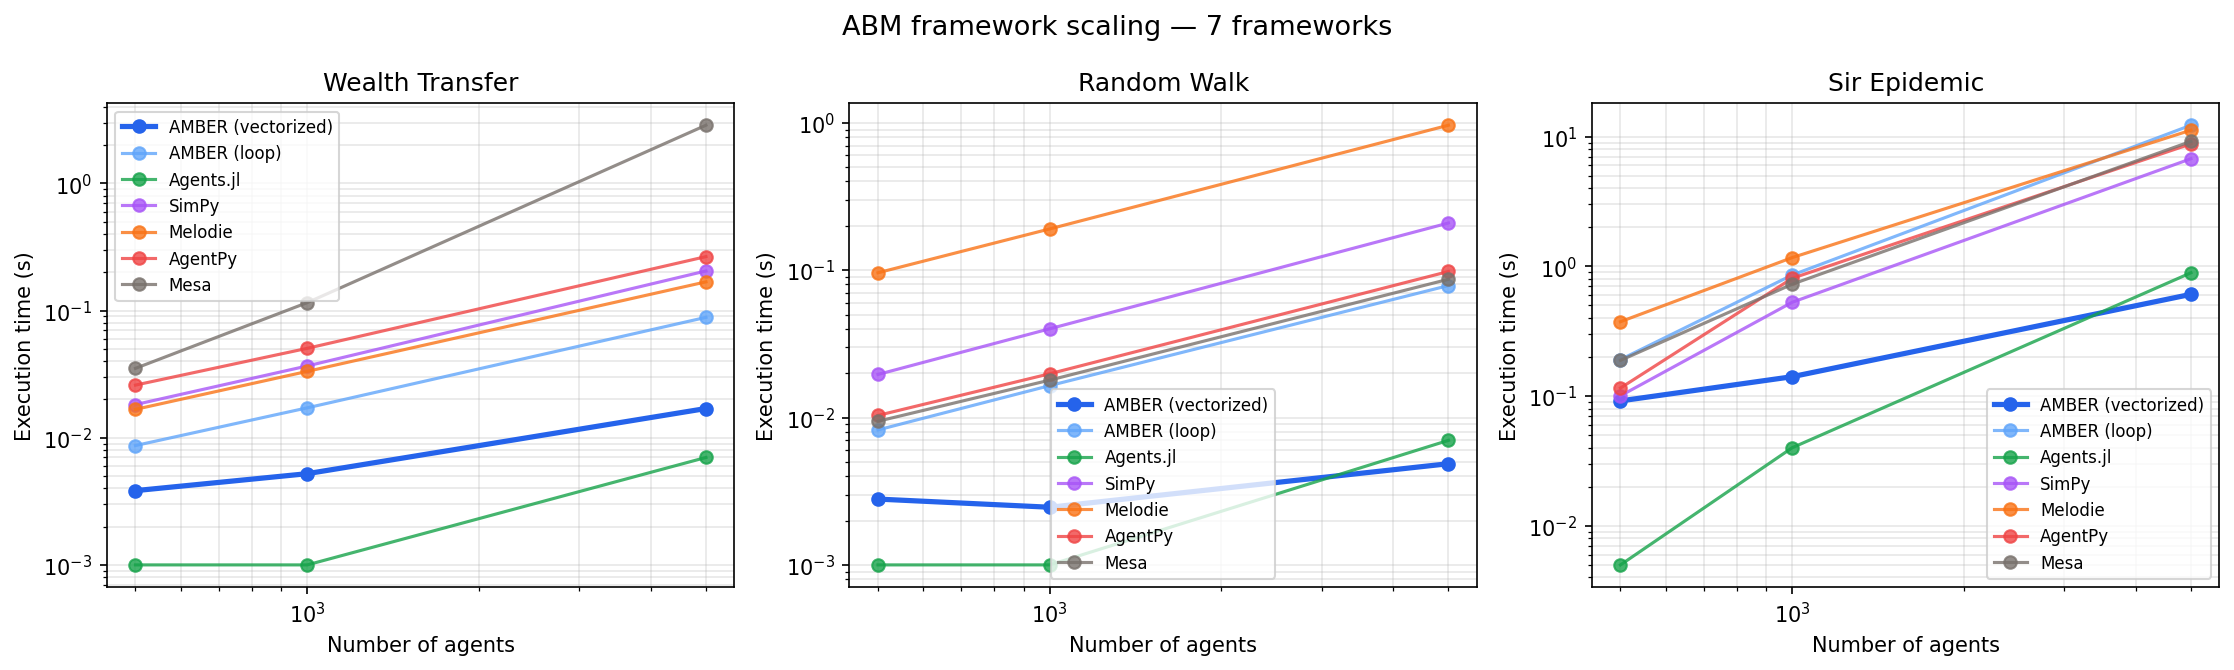
\includegraphics[width=\textwidth]{../benchmarks/results/scaling_chart_all.png}
    \caption{Execution time versus agent population size for three benchmark models, all seven frameworks. Lower is better. AMBER (vectorized) is the fastest Python-hosted implementation on every tested model; Agents.jl leads the cheap wealth-transfer and random-walk kernels, while AMBER leads the largest SIR workload.}
    \label{fig:scaling}
\end{figure}

\subsubsection{Execution Time}

Table~\ref{tab:results} reports execution time at all three tested population sizes. Values in milliseconds unless otherwise noted; bold entries mark the fastest framework per cell.

\begin{table}[H]
\centering
\caption{Execution time at 500, 1{,}000, and 5{,}000 agents over 50 simulation steps.}
\label{tab:results}
\small
\begin{tabular}{l rrr rrr rrr}
\toprule
 & \multicolumn{3}{c}{\textbf{Wealth Transfer}} & \multicolumn{3}{c}{\textbf{Random Walk}} & \multicolumn{3}{c}{\textbf{SIR Epidemic}} \\
\cmidrule(lr){2-4} \cmidrule(lr){5-7} \cmidrule(lr){8-10}
\textbf{Framework} & 500 & 1k & 5k & 500 & 1k & 5k & 500 & 1k & 5k \\
\midrule
AMBER (vectorized) & 4.4 & 6.4 & 21 & 2.7 & 2.7 & 6.2 & 95 & 119 & \textbf{687} \\
Agents.jl (Julia) & \textbf{0.6} & \textbf{1.4} & \textbf{7.2} & \textbf{0.1} & \textbf{0.3} & \textbf{1.6} & \textbf{4.2} & \textbf{36} & 808 \\
AMBER (loop) & 16 & 33 & 171 & 36 & 69 & 352 & 174 & 817 & 10{,}568 \\
SimPy & 18 & 38 & 218 & 25 & 48 & 261 & 119 & 497 & 5{,}506 \\
Melodie & 19 & 36 & 188 & 110 & 216 & 1{,}104 & 472 & 2{,}130 & 21{,}263 \\
AgentPy & 27 & 54 & 272 & 16 & 31 & 150 & 163 & 973 & 11{,}993 \\
Mesa & 261 & 996 & 23{,}917 & 16 & 28 & 141 & 250 & 1{,}150 & 17{,}967 \\
\bottomrule
\end{tabular}
\end{table}

\subsubsection{Speedup at 5{,}000 Agents}

Table~\ref{tab:speedups} re-expresses the 5{,}000-agent results as speedup ratios with AMBER (vectorized) as the baseline. Values greater than 1 indicate AMBER is faster; values less than 1 indicate the other framework is faster.

\begin{table}[H]
\centering
\caption{Speedup of AMBER (vectorized) vs each framework at $N = 5{,}000$ agents.}
\label{tab:speedups}
\begin{tabular}{lrrr}
\toprule
\textbf{Framework} & \textbf{Wealth Transfer} & \textbf{Random Walk} & \textbf{SIR Epidemic} \\
\midrule
Agents.jl (Julia)  & 0.3$\times$ (faster) & 0.3$\times$ (faster) & 1.2$\times$ \\
AMBER (loop)       & 8.0$\times$  & 56.8$\times$ & 15.4$\times$ \\
SimPy              & 10.2$\times$ & 42.0$\times$ & 8.0$\times$ \\
Melodie            & 8.8$\times$  & 178.0$\times$ & 30.9$\times$ \\
AgentPy            & 12.7$\times$ & 24.2$\times$ & 17.5$\times$ \\
Mesa               & 1117.6$\times$ & 22.8$\times$ & 26.1$\times$ \\
\bottomrule
\end{tabular}
\end{table}

\subsection{Analysis}

AMBER (vectorized) is the fastest Python-hosted framework on all three models and wins the largest SIR benchmark outright. Agents.jl wins the two cheaper microbenchmarks, where Julia's compiled dispatch has less fixed overhead than repeated Python-to-Polars calls. The story each row tells is slightly different.

\textbf{Random Walk.} Agents.jl wins at 1.6 ms vs AMBER's 6.2 ms because the per-step body is only two independent coordinate updates and a boundary clamp. There is little work for Polars to amortize, so Julia's compiled loop and low call overhead dominate. AMBER remains the fastest Python-hosted implementation, roughly 23$\times$ faster than Mesa at 5{,}000 agents.

\textbf{SIR Epidemic.} AMBER wins at 687 ms vs Agents.jl's 808 ms (1.2$\times$). The infection step is quadratic in population size because each infected agent must distance-test every susceptible agent. AMBER expresses this as a Polars cross join filtered by the squared-distance predicate, which runs as one compiled pipeline in Rust; Agents.jl does the same computation as a nested loop that the Julia compiler specializes per-call but which still processes one pair at a time at the assembly level. At 5{,}000 agents the Polars pipeline pays off; at smaller sizes Agents.jl wins because its per-call overhead is near zero.

\textbf{Wealth Transfer.} Agents.jl wins at 7.2 ms vs AMBER's 21 ms (3.0$\times$). The per-step work is so small --- one array comparison, one random draw per active agent, two scatter-adds --- that Polars' per-query overhead (query planning, Python--Rust boundary crossings, metadata bookkeeping) becomes the dominant cost. Julia's compiled dispatch wins the microbenchmark because there is essentially no computation for Polars to amortize over. Notably, AMBER is still roughly $13\times$ faster than every other Python-hosted framework on this workload, and the AMBER (loop) path alone beats Mesa by a factor of 140.

\textbf{AMBER loop vs Mesa on wealth transfer}: Mesa's 5{,}000-agent result (23.92 s) is 1118$\times$ slower than AMBER (vectorized) and 140$\times$ slower than AMBER (loop). This gap reflects Mesa 3.x's \texttt{AgentSet.shuffle\_do} materializing the full agent list per step for shuffle-ordered activation, compounded with the scheduler's per-agent dispatch overhead. The wealth-transfer workload happens to be a worst case for this pattern because every agent acts every step.

\textbf{When the Julia JIT wins.} The wealth-transfer and random-walk microbenchmarks are instructive: they establish the regime where a compiled JIT language has a structural advantage over a Python-hosted columnar framework. When the per-step work is $O(\mathrm{constant})$ per agent with little amortizable work, SIMD vectorization alone does not erase Python-to-Rust call overhead. Once the per-step computation becomes heavier, as in SIR, the columnar pipeline draws level with compiled Julia while remaining in Python.

\section{(4) Quality Control}

\subsection{Testing}

AMBER maintains an automated test suite of 245 unit and integration tests executed on every push to the \texttt{main} and \texttt{dev} branches via GitHub Actions. Coverage is tracked in CI, and tests are organised into:

\begin{itemize}
\item \textbf{Unit tests} (\path{tests/test_agent.py}, \path{tests/test_model.py}, \path{tests/test_sequences.py}, \path{tests/test_population.py}, and \path{tests/test_base.py}) covering the view API's attribute read/write protocol, the write-buffer flush semantics, \texttt{add\_agents} bulk creation, filtered and scatter view construction, and all legacy list-style compatibility surfaces.
\item \textbf{Environment tests} (\path{tests/test_environments.py}) covering grid, continuous-space, and network environments, including a regression guard for a torus-wrap neighbour-deduplication bug fixed as part of this release.
\item \textbf{Integration tests} (\path{tests/test_integration.py}) covering end-to-end simulation workflows. The file deliberately keeps two class suites: \texttt{TestFullSimulationWorkflows} exercises the legacy per-agent loop path as a backwards-compatibility regression guard, while \texttt{TestVectorizedWorkflows} exercises the view API idiom.
\item \textbf{Optimisation tests} (\path{tests/test_optimization.py}) covering the grid-, random-, Bayesian-, and SMAC-based calibration paths.
\end{itemize}

Continuous integration runs on Ubuntu, macOS, and Windows across Python 3.10, 3.11, and 3.12. The documentation is built with Sphinx under \texttt{-W --keep-going} (warnings treated as errors) as part of the release workflow.

\subsection{Correctness of Benchmark Implementations}

Runtime numbers are meaningful only if every framework is computing the same thing. Before any timing run, AMBER executes each framework implementation against a dedicated correctness script, \path{benchmarks/correctness_check.py}, that checks per-model output invariants:

\begin{itemize}
\item \textbf{Wealth transfer}: total wealth must equal $N \cdot w_{init}$ at every step (Boltzmann conservation).
\item \textbf{Random walk}: all agent coordinates must lie within the configured world bounds.
\item \textbf{SIR epidemic}: the cardinalities $|S| + |I| + |R|$ must equal $N$ at every step, and the initial infected count must match the configured parameter.
\end{itemize}

This audit surfaced multiple benchmark defects: SimPy's wealth-transfer helper used a race-prone event update, SimPy lacked random-walk boundary clamping, SimPy's SIR helper hardcoded every agent as initially infected, Agents.jl used a hardcoded step count, SimPy, Melodie, and Agents.jl used a different movement kernel from AMBER, AgentPy, and Mesa, and Mesa's benchmark model did not route seeded runs through Mesa's model RNG. The corrected evaluation in Section~\ref{sec:evaluation} reflects every framework passing the relevant invariants.

\section{(5) Availability}

\subsection{Operating System}

Linux, macOS, and Windows.

\subsection{Programming Language}

Python $\geq 3.10$.

\subsection{Additional System Requirements}

None beyond a standard Python 3 installation. No GPU required.

\subsection{Dependencies}

Required: Polars $\geq 1.0$, NumPy $\geq 1.20$, NetworkX $\geq 2.5$, Matplotlib $\geq 3.3$, Seaborn $\geq 0.11$, scikit-optimize $\geq 0.9$. Optional: SMAC $\geq 2.0$ and ConfigSpace $\geq 0.7$ (advanced calibration); plotly and ipywidgets (interactive examples). Development: pytest, pytest-cov, Sphinx, sphinx-rtd-theme.

\subsection{List of Contributors}

Anh-Duy Pham (University of W\"{u}rzburg) is the primary author and maintainer. A complete list of contributors is available in the git history at \url{https://github.com/a11to1n3/AMBER/graphs/contributors}.

\subsection{Software Location}

\begin{description}
\item[Code repository.] Name: AMBER. Identifier: \url{https://github.com/a11to1n3/AMBER}. Licence: BSD 3-Clause. Date published: 2024. Version published at time of writing: \texttt{v0.3.1}.

\item[Archive.] Name: Zenodo. Identifier: \texttt{10.5281/zenodo.XXXXXXX} (to be minted on acceptance via the GitHub--Zenodo integration). Licence: BSD 3-Clause. Publisher: Anh-Duy Pham. Version published: \texttt{v0.3.1}. Date published: May 2026.
\end{description}

\subsection{Language}

The software is written in Python. All user-facing documentation, source comments, and test names are in English.

\section{(6) Reuse Potential}

AMBER is designed as a general-purpose ABM framework. Three categories of users are targeted.

\textbf{Domain scientists building mid-to-large-scale models.} Epidemiologists simulating disease transmission across contact networks, ecologists modelling species distributions or predator-prey dynamics, economists studying market formation or financial contagion, and social scientists investigating opinion dynamics can all express their models in AMBER using the view API with population sizes comfortably in the tens of thousands. Existing Mesa or AgentPy models port with relatively minor edits: the \texttt{Model}/\texttt{Agent} class hierarchy is preserved, and the main code change is rewriting population-wide updates as \texttt{agents.where(...)} expressions instead of per-agent loops. The OOP escape hatch lets per-agent logic that does not vectorise---graph traversal, Schelling-style satisfaction checks, or rule-based strategic behaviour---coexist with the vectorised core.

\textbf{Method developers extending the columnar paradigm.} The \texttt{Population} class (the columnar backend) and the view-API base class (\texttt{\_BaseView}) are deliberately documented as extension points. Researchers exploring novel ABM architectures---for example, GPU offload via cuDF, cluster-scale simulation via Arrow Flight, or integration with automatic-differentiation libraries---can reuse AMBER's data model without reinventing the state management layer. The three-view taxonomy (full / filtered / scatter) has room for extension (windowed views for time-series analyses, graph-neighbourhood views for networked models).

\textbf{Educators teaching ABM.} The legacy per-agent API remains fully supported and is the natural introduction path for students new to agent-based thinking. Once a model is working, the same class can be incrementally migrated to the view API as a lesson in vectorisation and performance engineering. The documentation (\url{https://amber.readthedocs.io}) provides a quickstart tutorial, a full walkthrough of three canonical models, and API reference material generated from source docstrings.

Support is provided via the GitHub issue tracker (\url{https://github.com/a11to1n3/AMBER/issues}). Contributions in the form of bug reports, pull requests, and new examples are welcome; the contributing guide in the repository describes the development workflow and the code-review criteria.

\section*{Acknowledgements}

We gratefully acknowledge the open-source communities behind Polars and Apache Arrow, whose work on high-performance columnar data processing forms the foundation of this project.

\section*{Funding Statement}

This work received no specific grant from any funding agency in the public, commercial, or not-for-profit sectors.

\section*{Competing Interests}

The author declares no competing interests.

\bibliographystyle{plainnat}
\bibliography{paper}

\end{document}
